\chapter{Demonstrations of Full Data Abstraction}
\lhead{\emph{Demonstrations of Full Data Abstraction}}

\begin{figure}[h]
    \begin{center}
    \begin{tabular}{ c c }
        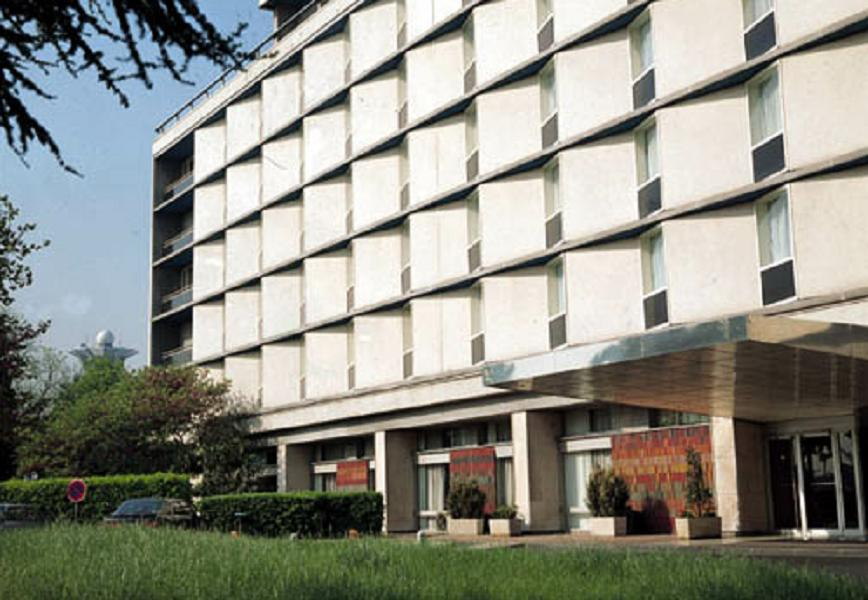
\includegraphics[width=0.45\textwidth]{Figures/building.jpg} &
        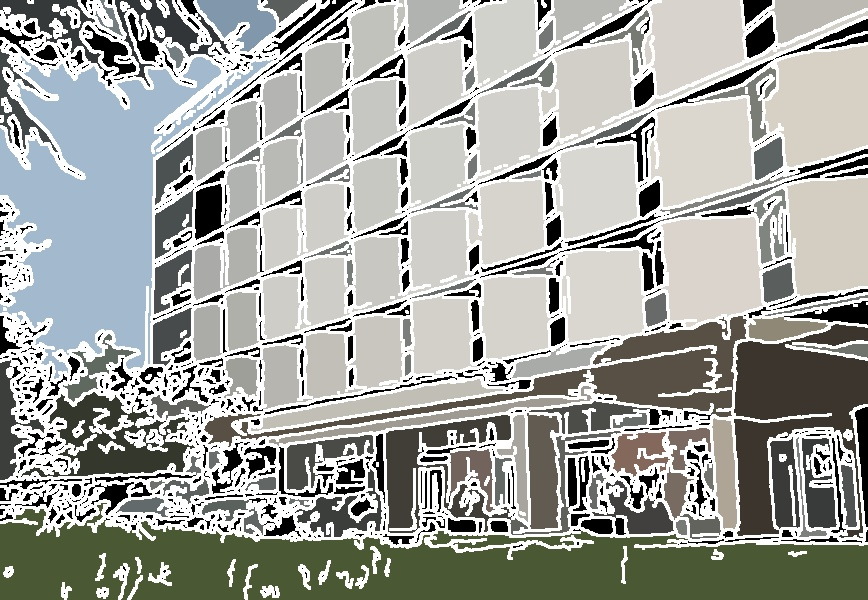
\includegraphics[width=0.45\textwidth]{Figures/Final.jpg} \\
    \end{tabular}
    \caption[Demonstration of full abstraction process]{Demonstration of full abstraction process. The final parameters and methods (of those under discussion) are a blur kernel of 5x5, a low threshold of 25 (for this example), Sobol seed point generation, and averaging via preliminary flood fill. It can be seen that most areas of the image are being effectively edge detected and flood filled with the correct colours; however, some areas are hard to interpret such as around the bushes in the bottom left, and some spaces have been left unfilled such as the panel below the top left corner of the building. These issues are minimal though, therefore leading me to conclude that the process is effective at producing recognisable abstractions of the input images.}
    \label{fig:Final}
    \end{center}
\end{figure}
        
\begin{figure}[ht]
    \begin{center}
    \begin{tabular}{ c c }
        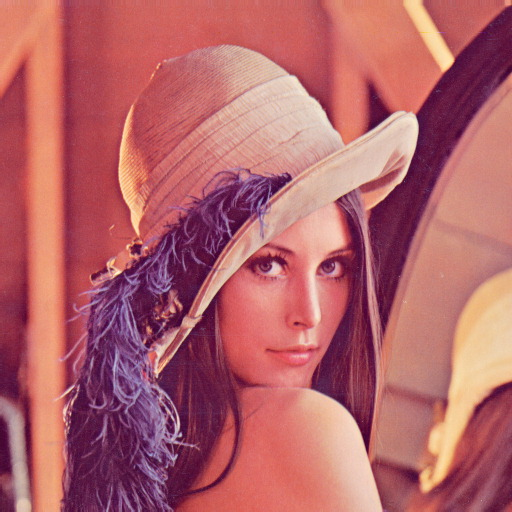
\includegraphics[width=0.43\textwidth]{Figures/lena.jpg} &
        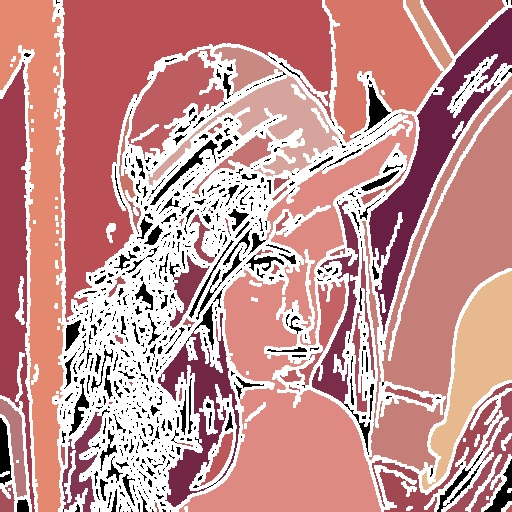
\includegraphics[width=0.43\textwidth]{Figures/lenaDA.jpg} \\
        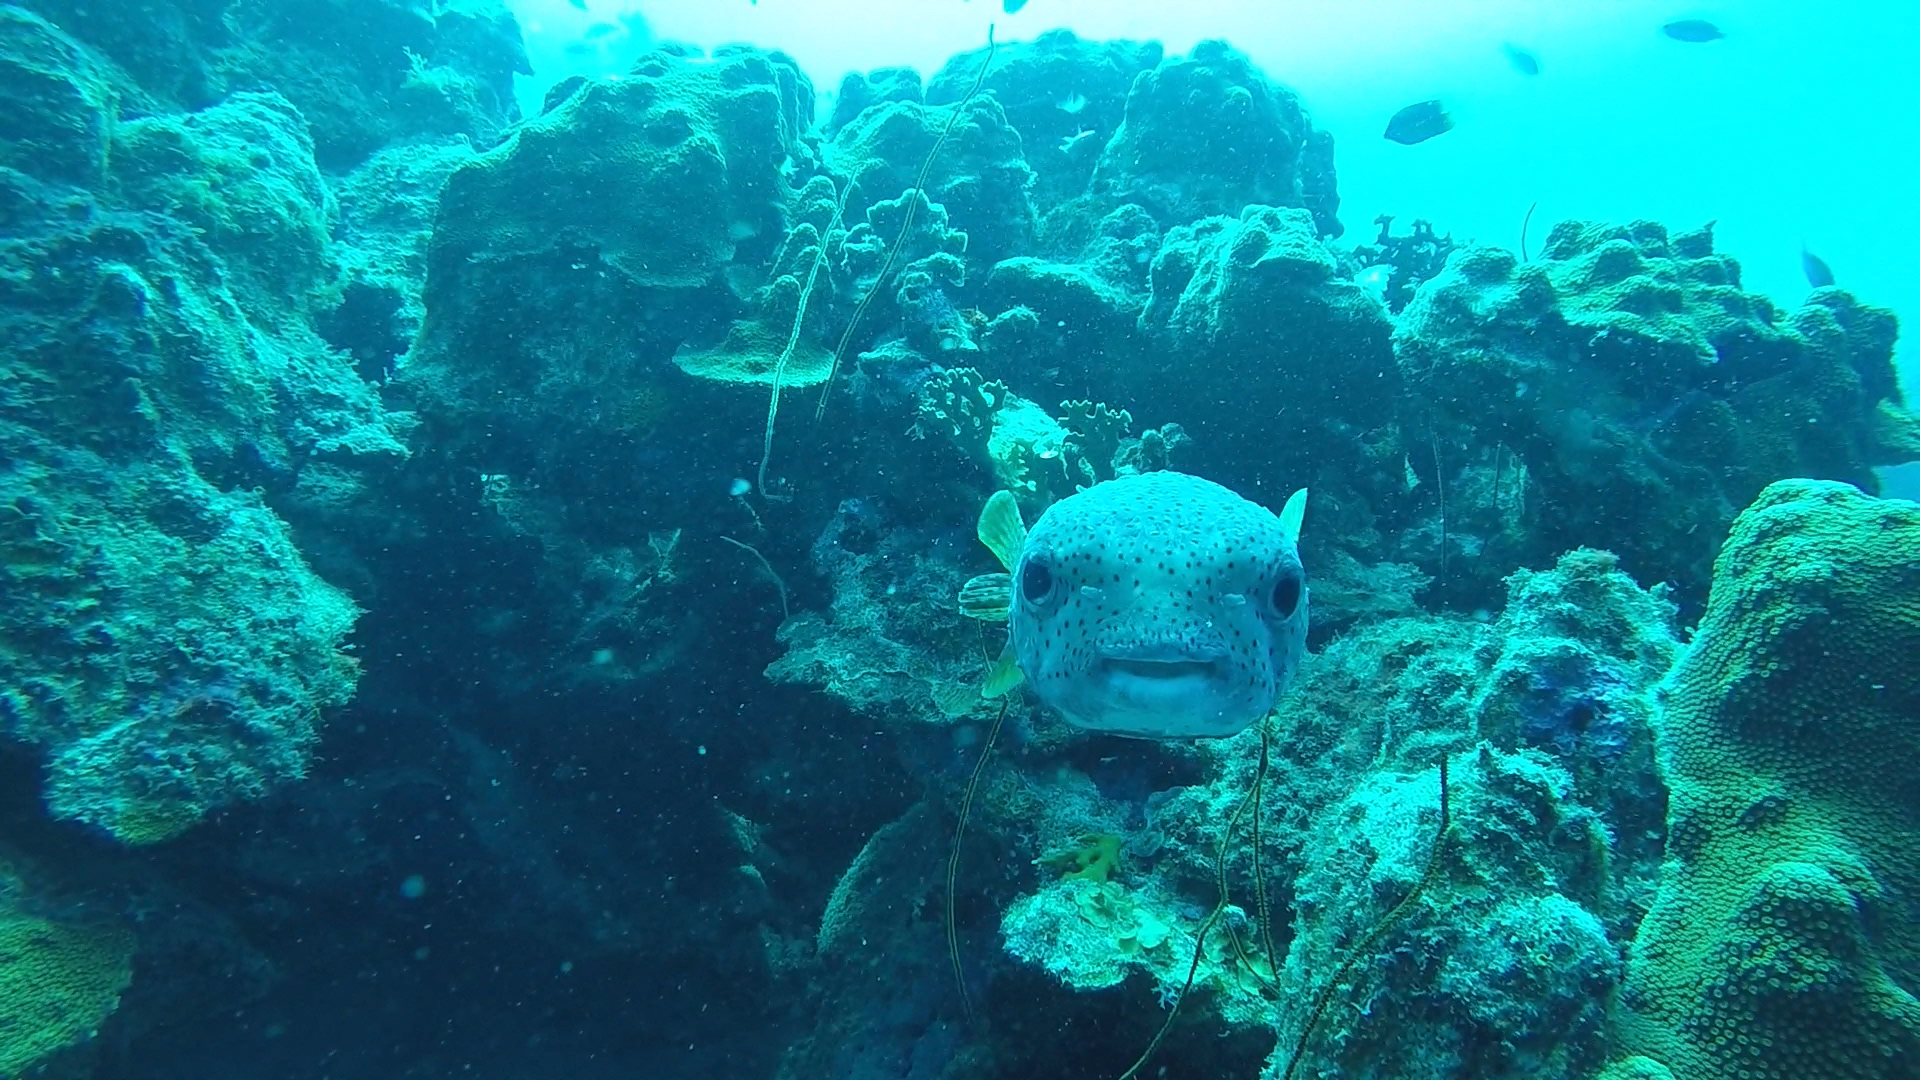
\includegraphics[width=0.43\textwidth]{Figures/pufferfish6.jpg} &
        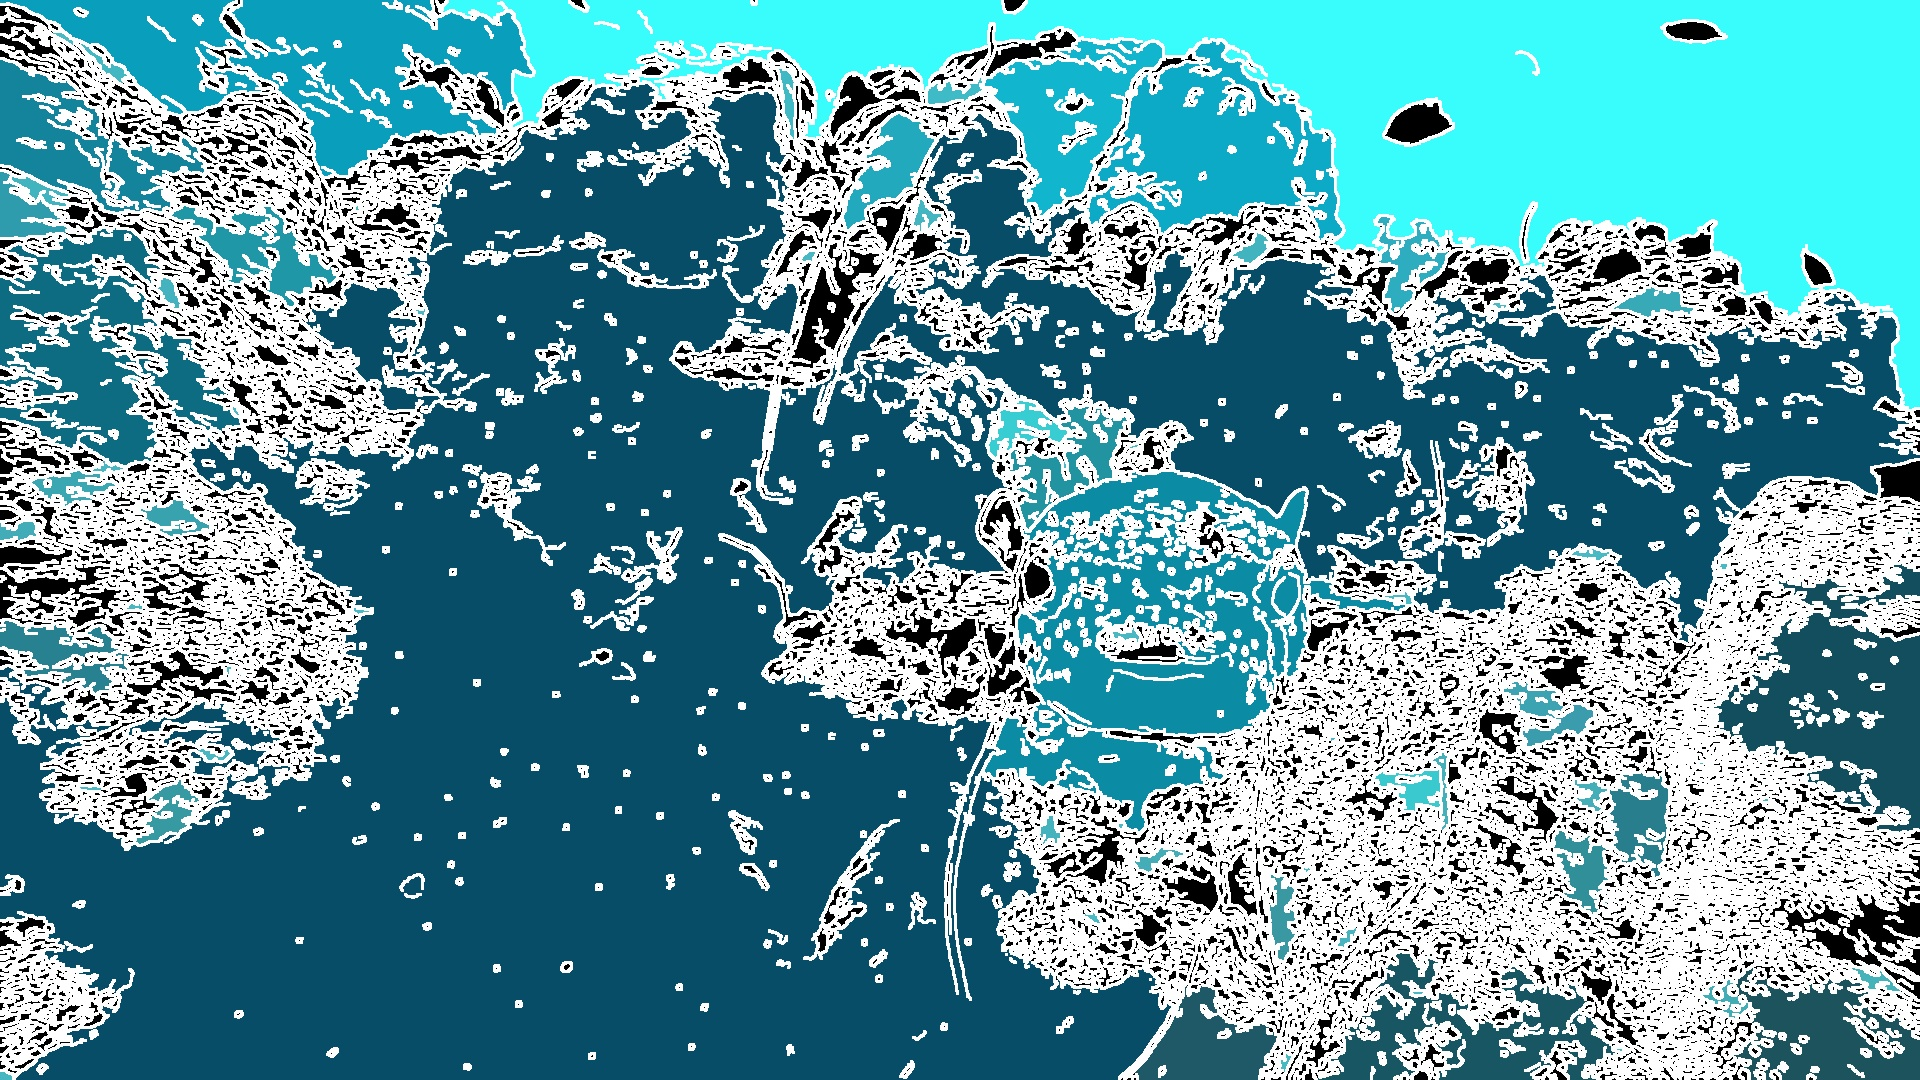
\includegraphics[width=0.43\textwidth]{Figures/pufferfishDA.jpg} \\
        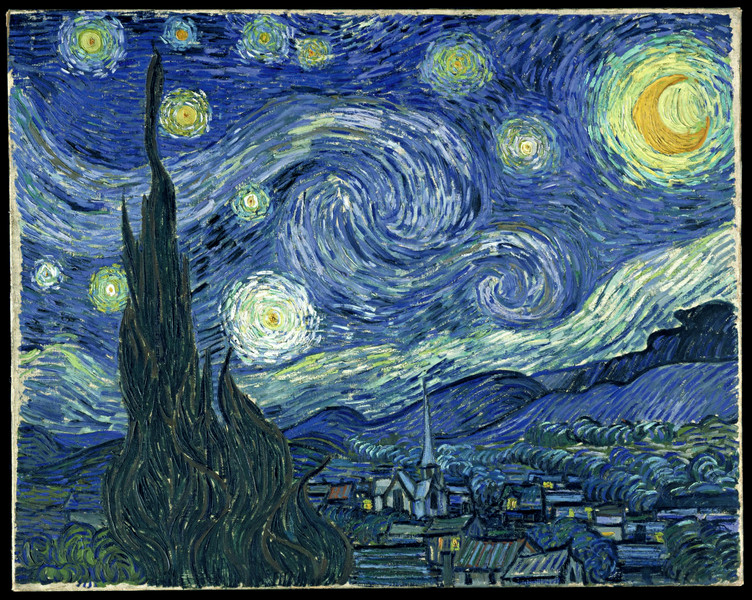
\includegraphics[width=0.43\textwidth]{Figures/starry_night.jpg} &
        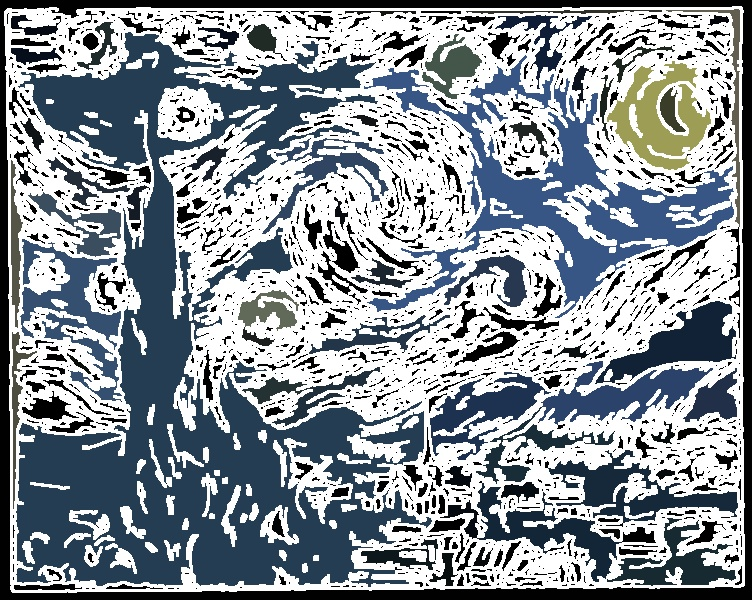
\includegraphics[width=0.43\textwidth]{Figures/starry_nightDA.jpg} 
    \end{tabular}
    \caption[Additional examples of the full abstraction process]{Additional examples of the full abstraction process. The top image (provided by OpenCV) is very simple, so the abstraction gives clean and easily recognisable results. The middle image (provided by fellow student Tom Darlison) was selected due to its limited colour palette and poor focus to test the limits of the process. While the image has mostly filled to a single colour, the pufferfish, rocks, coral, background fish, and open water are all identifiable. The bottom image (provided by OpenCV) was selected due to the extreme number of edges, due to the very clear brush strokes. Once the Canny threshold was turned down considerably, the result was recognisable as Starry Night, though much of the image has been overwhelmed by the edge detection lines. It can be concluded from these tests that the data abstraction process is effective at producing recognisable images, however the difficulty in interpreting the abstracted images is heavily dependant on the focus and complexity of the image.}
    \label{fig:FinalExtras}
    \end{center}
\end{figure}